\section{Descrizione generale}

\subsection{Obiettivi del progetto}
Il progetto \NomeProgetto{} ha come obiettivo finale creare una piattaforma che consenta agli sviluppatori di fare il deploy di funzioni JavaScript, preoccupandosi solamente della relativa codifica e non dell'architettura sottostante. Allo stesso tempo, tali funzioni vengono messe a disposizione agli altri utenti, che possono eseguirle e pagare secondo un modello CaaS (Computation as a Service), cioè solamente per il tempo e le risorse richieste dalla loro esecuzione.

\subsection{Funzionalità del prodotto}
L'applicativo deve fornire agli sviluppatori la possibilità di caricare nel cloud le proprie funzioni e renderle disponibili secondo la modalità FaaS (Function as a Service). Gli utenti finali possono usufruire di tali servizi pagando una certa quantità di ETH, e gli sviluppatori non si devono quindi preoccupare della gestione dell'infrastruttura alla base dei servizi, ma possono guadagnare all'esecuzione di ogni funzione da loro caricata. \\
Nello specifico:
	\begin{itemize}
		\item gli utenti finali e gli sviluppatori possono:
		\begin{enumerate}[a.]
			\item autenticarsi all'interno della rete Ethereum;
			\item eseguire una funzione presente nella piattaforma e visualizzarne i risultati;
			\item elencare tutte le funzioni disponibili nella piattaforma;
			\item visualizzare i dettagli di una determinata funzione;
			\item visualizzare la propria cronologia di esecuzione di funzioni;
			\item ricercare funzioni in base ad un termine di ricerca.
		%	\item visualizzare i dettagli relativi all'esecuzione di una specifica funzione;
		\end{enumerate}

		\item gli sviluppatori possono:
		\begin{enumerate}[a.]
			\item caricare all'interno della piattaforma delle proprie funzioni Javascript;
			\item eliminare una funzione da loro precedentemente caricata;
			\item modificare le informazioni e il codice relativo ad una loro funzione.
		\end{enumerate}
	\end{itemize}

	\begin{landscape}
		\subsection{Diagramma di package del prodotto}
		\begin{figure}[H]
			\centering
			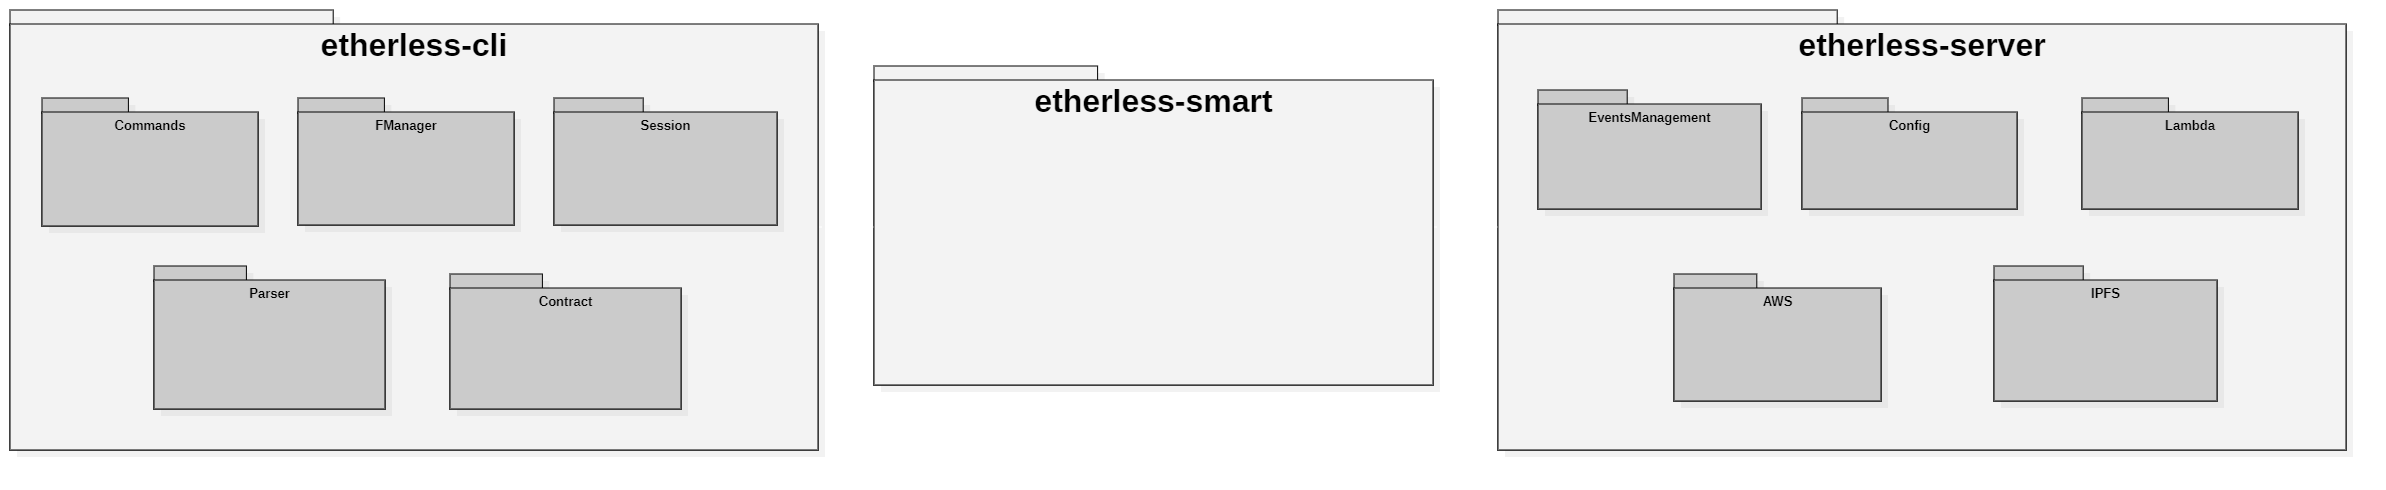
\includegraphics[width=1.4\textwidth]{././diagrammi/generali/Etherless_package.png}
			\caption{Diagramma di package del prodotto}
		\end{figure}

	\end{landscape}
\newpage
\subsection{Diagrammi di attività}
	La comunicazione tra i tre moduli che costituiscono il prodotto segue due diversi pattern in base al tipo di operazione da eseguire.
	\paragraph{Primo pattern di comunicazione}
		Questo pattern di comunicazione riguarda tutte le funzionalità che necessitano di comunicare con la componente server per completare la propria esecuzione. Dato che il modulo smart non é in grado di eseguire chiamate esterne, tutte le comunicazioni uscenti da questo modulo sono sotto forma di eventi emessi nella rete Ethereum, di cui gli altri moduli si mettono in ascolto. \\ Degli esempi di funzionalità che seguono di questo pattern di comunicazione sono:
		\begin{itemize}
			\item l'esecuzione di una funzione caricata sulla piattaforma \NomeProgetto{};
			\item il deployment di una funzione.
		\end{itemize}
		\begin{figure}[H]
			\centering
			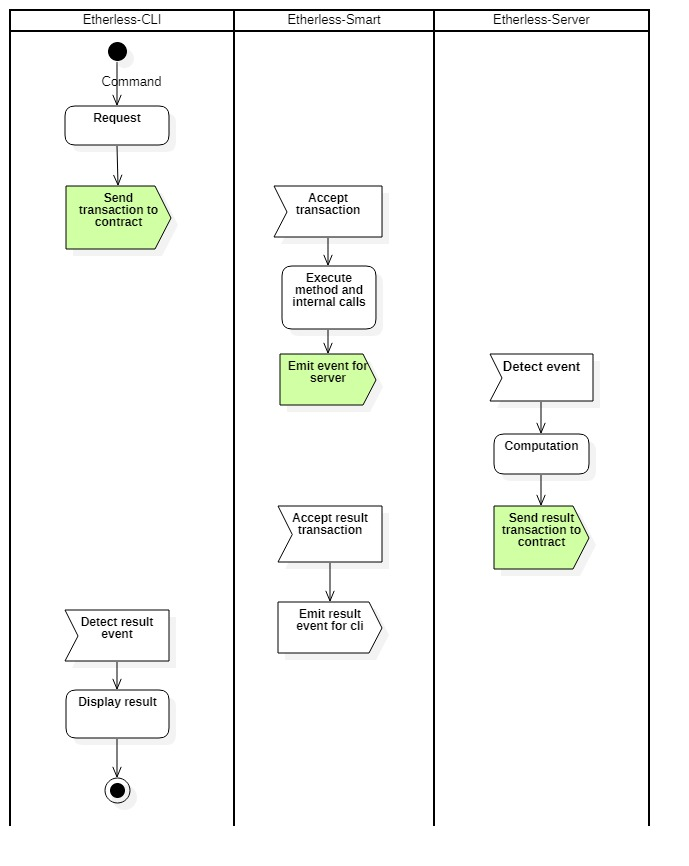
\includegraphics[width=0.7\textwidth]{././diagrammi/generali/activity_diag_pattern2.jpg}
			\caption{Diagramma di attività per il primo pattern di comunicazione}
		\end{figure}
	\paragraph{Secondo pattern di comunicazione}
		Nel caso in cui sia necessario recuperare informazioni riguardanti una o più funzioni, il modulo cli ottiene questi dati attraverso una chiamata alle funzioni del modulo smart, senza necessitare della partecipazione del modulo server.\\  Degli esempi di funzionalità che seguono di questo pattern di comunicazione sono:
		\begin{itemize}
			\item visualizzazione della lista delle funzioni;
			\item visualizzazione delle informazioni dettagliate di una funzione.
		\end{itemize}
	\begin{figure}[H]
		\centering
		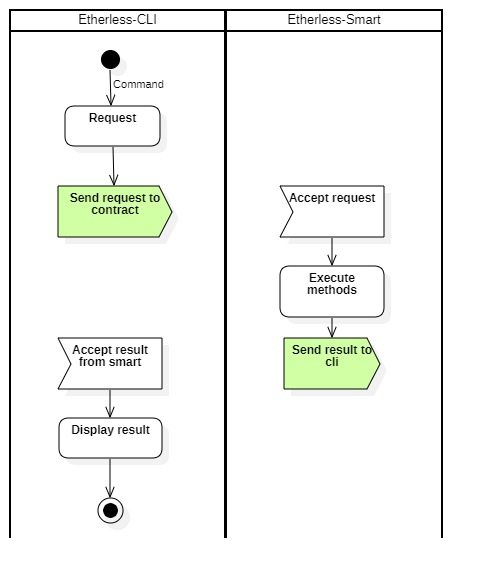
\includegraphics[width=0.8\textwidth]{././diagrammi/generali/activity_diag_pattern1.jpg}
		\caption{Diagramma di attività per il secondo pattern di comunicazione}
	\end{figure}
